\vspace{-0.4cm}
\section{Atypical Samples in Adversarial Training}\label{sec:pre}
\vspace{-0.2cm}
In this section, we attempt to understand adversarial training's behavior by studying its relation with the memorization effect. The discussions are mainly based on PGD-adversarial training~\cite{madry2017towards} on CIFAR~100. Implementation details are shown in Appendix~\ref{app:pre} where we also report the results in more datasets, i.e., CIFAR~10 and Tiny~ImageNet~\cite{le2015tiny}, and we make consistent observations.

\vspace{-0.2cm}
\subsection{Adversarial Robustness of Atypical Samples is Harder to Generalize}\label{sec:pre1}
\begin{figure}[t]
\centering
\hspace*{-1cm}
\subfloat[Clean (left) \& Adv Acc. (right) under ResNet18.]{
\label{fig:harder1}
\begin{minipage}[c]{0.55\textwidth}
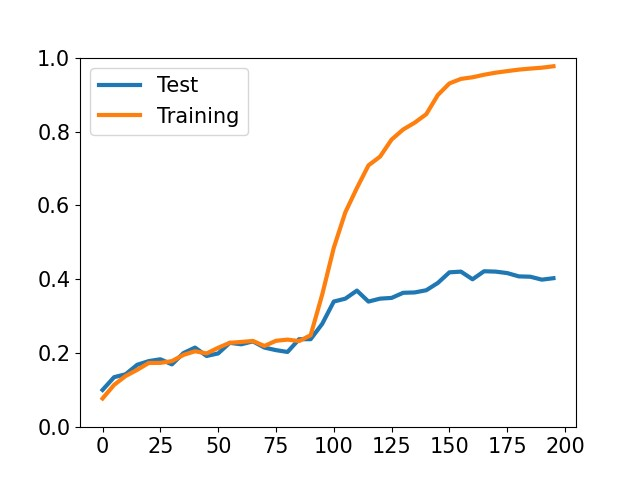
\includegraphics[width = 0.5\textwidth]{figures/clean_rare_cifar.jpg}%
\hfill
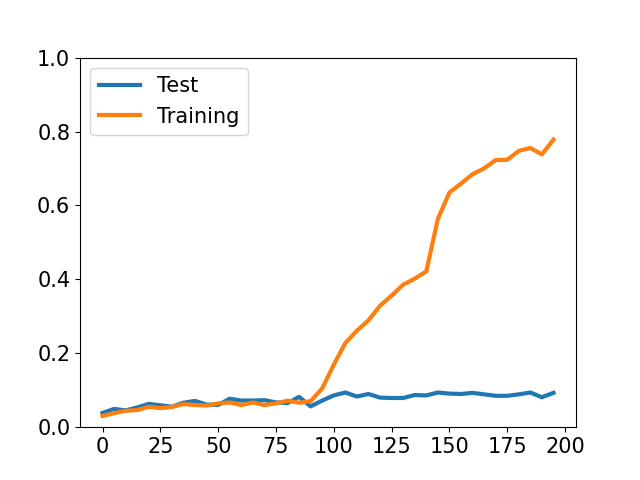
\includegraphics[width = 0.5\textwidth]{figures/adv_rare_cifar100.png}
\end{minipage}
}
\hspace*{-0.4cm}
\subfloat[Clean (left) \& Adv Acc. (right) under WRN28.]{
\label{fig:harder3}
\begin{minipage}[c]{0.55\textwidth}
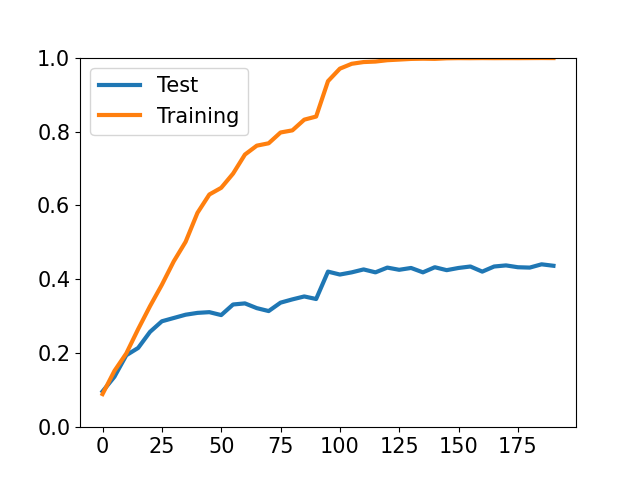
\includegraphics[width = 0.5\textwidth]{figures/wrn_clean_rare_cifar100.png}%
\hfill
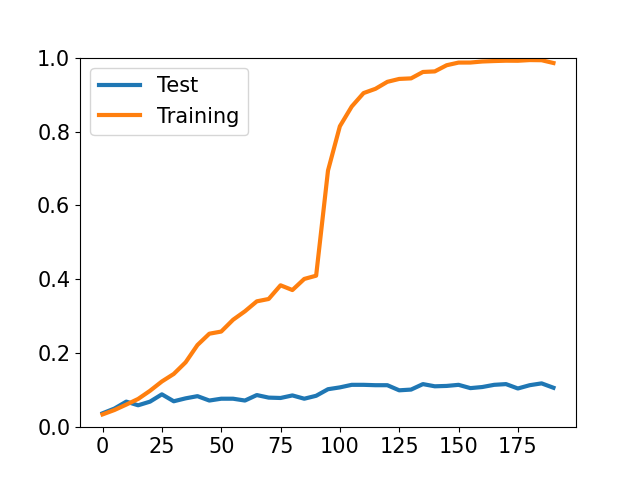
\includegraphics[width = 0.5\textwidth]{figures/wrn_adv_rare_cifar100.png}
\end{minipage}
}
\caption{Clean Accuracy and Adversarial Accuracy on \textbf{Atypical} Set of CIFAR100}
\vspace{-0.5cm}
\label{fig:rare_benefit}
\end{figure}
In this subsection, we first check whether fitting atypical samples in adversarial training can effectively help the model correctly and robustly predict the atypical samples in the test set. We apply PGD adversarial training~\cite{madry2017towards} on original CIFAR~100 dataset for 200 epochs and evaluate the model's clean accuracy and adversarial accuracy on training atypical set $\mathcal{D}_\text{atyp}=\{x_i \in \mathcal{D}: \text{mem}(x_i)> 0.15\}$ and its corresponding test atypical set $\mathcal{D}_\text{atyp}' = \{x'_j \in \mathcal{D}': \text{infl}(x_i,x'_j)> 0.15, \text{for } \forall x_i\in \mathcal{D}_\text{atyp}\}$. In Fig.~\ref{fig:rare_benefit}, we report the algorithm's performance (clean \& adv. acc.) on these atypical sets along with the training process. From the results, we observe that both ResNet18 and WRN28 are capable to memorize all clean atypical samples and most adversarial atypical samples, since they both achieve $\approx100\%$ clean accuracy and high adversarial accuracy ($\approx80\%$ and $100\%$, respectively) on the training atypical set. 
As the training goes, the models' clean accuracy on the test atypical set gradually improves and finally approaches 40\%. 
However, their adversarial robustness keep constant around 10\% from the beginning epochs to the last ones, no matter how high the training performance is. 
These results suggest that the memorizing atypical samples in adversarial training may only improve their test clean accuracy, but hardly help their adversarial robustness. Recall that in CIFAR100, atypical set $\mathcal{D}_\text{atyp}$ (with memorization value > 0.15) covers 40\% samples of the whole dataset. Completely failing on the adversarial robustness of atypical samples could be one important reason that contributes to the poor robustness generalization of DNNs~\cite{rice2020overfitting}.

As the previous theoretical study~\cite{schmidt2018adversarially} states, for a model to have good robustness generalization performance, it always demands a training set with much larger amount of samples, than a model to have good clean accuracy generalization. In our case, the sub-population of each particular atypical sample has very low frequency to appear in the training set, and it is always deviated from the main sub-population. Thus, in the sub-population of this atypical sample, it is equivalent to a classification task based on an extremely small dataset, with one or a few training samples given. Therefore, the adversarial robustness of atypical samples can be extremely hard to generalize. 
%\han{Note that the sub-population of each particular atypical sample has very low frequency to appear in the training set and it is always deviated from the main sub-population. Thus, for DNNs to classify the samples in the sub-population of this atypical sample, it is equivalent to a claication }


